\begin{partbacktext}
\part{Fundamentos}
En la primera parte de la monografía presentaremos los conceptos fundamentales para modelar y simular los problemas de las ecuaciones en diferencias, a veces, mal llamado \emph{relaciones de recurrencias}. En el capítulo $1$ presentaremos los modelos fundamentales y las ecuaciones en diferencias. Discutiremos la relación de \emph{Ackermann}
\end{partbacktext}
%\chapauthor{Autor}
%\chapsubtitle{Subtítulo}
\chapter{Introducción}
\abstract{En este capítulo introducimos las relaciones de recurrencia. Estas son ecuaciones que definen de manera recursiva, a través de funciones adecuadas, los términos que aparecen en una sucesión real o compleja. La primera sección trata algunos ejemplos bien conocidos que muestran cómo estas relaciones pueden surgir en la vida real, por ejemplo, el problema de la Torre de Hanoi o el problema de Flavio Josefo. Luego, dedicamos una gran parte del capítulo a las ecuaciones en diferencias, es decir, $\Delta x_{n}$, donde $f$ es una función de valor real: en este contexto, los métodos más estudiados son el de Euler y Runge-Kutta. Estudiamos a fondo el caso que pueden ser usados para resolver ecuaciones diferenciales ordinarias. La última parte del capítulo está dedicada al célebre teorema del Polinomio minimal, que afirma que la raíz de un implica la solución: así le damos al estudiante el sabor de un sistema dinámico, esa noción no se desarrolla explícitamente en la monografía.}
%\chaptermark{xd}
\section{Relación de Recurrencia}
En esta sección presentamos a nuestros lectores las nociones básicas subyacentes de las relaciones de recurrencia, así como varios ejemplos de tales relaciones.

Una relación de recurrencia es una familia numerable de ecuaciones que definen sucesiones en modo recursivo. Aquellas sucesiones que así surgen se llaman \emph{soluciones de la recurrencia}, dependiendo de uno o más \emph{valores iniciales}: cada término que sigue al valor inicial en tales sucesiones es definida como una función de los términos anteriores.

\begin{example}{Relación de recurrencia real}\leavevmode
	\begin{enumerate}
		\item El sistema de ecuaciones con coeficientes reales en la colección infinita de incógnitas $x_{0},x_{1},\ldots,x_{n,\ldots}$ \[  \ccases{x_{1}&=3x_{0}\\x_{2}&=3x_{1}\\\vdots&=\vdots\\x_{n+1}&=3x_{n}\\\vdots&=\vdots} \] lo que puede indicarse más concisamente por $x_{n+1}=3x_{n},n\geq0$, es una \emph{relación de recurrencia}. La sucesión ${\left(3^{n}\right)}_{n\geq0}$ es una solución de la recurrencia dada con valor inicial $x_{0}=1$. Es fácil de convencerse a uno mismo que en general, para cualquier número real $c\in\mathds{R}$, la sucesión ${\left(c3^{n}\right)}_{n\geq0}$ es la única solución de la \emph{recurrencia} dado la condición inicial $x_{0}=c$.
		\item Con el cuidado adecuado es fácil verificar que la sucesión real \[ x_{0}=1,\quad x_{1}=1,\quad x_{2}=2,\quad x_{3}=2,\quad x_{4}=4,\quad\ldots\quad,x_{7}=4,\quad,\ldots,\quad x_{2^{m}}=2^{m},\quad\ldots \] es la solución de la \emph{relación de recurrencia} con coeficientes reales \[ x_{n}=\ccases{2x_{n/2},&\text{si }n\geq2\text{ es par},\\x_{n-1},&\text{si }n\text{ es impar},} \] con la condición inicial $x_{0}=1$.
		\item La sucesión real \[ x_{0}=2,\quad,x_{1}=1,\quad x_{2}=2^{1/2},\quad x_{3}=1,\quad\ldots,x_{2m-1}=1,\quad,x_{2m}=2^{1/2^{m}},\quad\ldots \] es la solución de la \emph{relación de recurrencia} con coeficientes reales \[ x_{n}=\sqrt{x_{n}-2},\quad n\geq2, \] y condiciones iniciales $x_{0}=2$ y $x_{1}=1$.
	\end{enumerate}
\end{example}

La pregunta que ahora surge naturalmente es la de definir relaciones generales de recurrencia. Buscamos exponer de manera rigurosa lo que acabamos de inferior de los ejemplos anteriores.

\begin{definition}[Relación de recurrencia]\index{Relación de recurrencia!definición}\label{def:recurrence}
	Una \textbf{relación de recurrencia} en las incógnitas $x_{i}$, $i\in\mathds{N}$, es una familia de ecuaciones
	\begin{equation*}
	x_{n}=f_{n}\left(x_{0},\ldots,x_{n-1}\right),\quad n\geq r,
	\end{equation*}
	donde $r\in\mathds{N}_{\geq1}$, y ${\left(f_{n}\right)}_{n\geq r}$ son funciones
	\begin{equation*}
	f_{n}\colon D_{n}\rightarrow\mathds{R},\quad D_{n}\subseteq\mathds{R}^{n},\qquad\text{o}\qquad f_{n}\colon D_{n}\rightarrow\mathds{C},\quad D_{n}\subseteq\mathds{C}^{n}.
	\end{equation*}
	Dependiendo del caso encontrado, las llamaremos \textbf{recurrencias reales}\index{Relación de recurrencia!real} o \textbf{recurrencias complejas}\index{Relación de recurrencia!compleja}. Las incógnitas $x_{0},\ldots,x_{r-1}$ son llamadas \textbf{libres}. El número $r$ es el \emph{orden de la relación}\index{Relación de recurrencia!orden}.
	
	Al reemplazar $n$ por $n+r$, la relación de recurrencia de orden $r$
	\begin{equation*}
	x_{n}=f_{n}\left(x_{0},\ldots,x_{n-1}\right),\quad n\geq r,
	\end{equation*}
	puede también escribirse como
	\begin{equation*}
	x_{n+r}=f_{n+r}\left(x_{0},\ldots,x_{n+r-1}\right),\quad n\geq0.
	\end{equation*}
\end{definition}

\begin{definition}[Solución de una recurrencia]\index{Relación de recurrencia!solución}
	Una sucesión $ \LEFTRIGHT\{\}{a_{n}}_{n\in\mathds{N}}$ es una \textbf{solución} de la relación de recurrencia de orden $r$
	\begin{equation}
	x_{n}=f_{n}\left(x_{0},\ldots,x_{n-1}\right),\quad n\geq r,
	\end{equation}
	con $f_{n}\colon D_{n}\rightarrow\mathds{R}$, $D_{n}\in\mathds{R}^{n}$, sii
	\begin{equation*}
	\LEFTRIGHT\{\}{a_{0},\ldots,a_{n-1}}\in D_{n},\implies a_{n}=f_{n}\left(a_{0},a_{1},\ldots,a_{n-1}\right)\quad\forall\,n\geq r.
	\end{equation*}
\end{definition}

La sucesión $\left\{a_{0},\ldots,a_{r-1}\right\}$ de valores asignados para las $r$ incógnitas libres es llamada la $r$--sucesión de \textbf{valor inicial} o de las \textbf{condiciones iniciales} de la solución. Definimos la \textbf{solución general real} (respectivamente \textbf{compleja}) de la sucesión como la familia de todas las soluciones con elementos que pertenece a $\mathds{R}$ (respectivamente en $\mathds{C}$).

\begin{example}{Relación de recurrencia de orden $1$}
	Considere la relación de recurrencia de primer orden definida por \[x_{n}=\frac{1}{x_{n-1}-1},\quad n\geq1.\]

	La $1$--sucesión $\left\{2\right\}\in D_{0}$ no es una sucesión de valor inicial de una solución, en efecto, $2$ pertenece al dominio de $f_{0}\left(x\right)=\frac{1}{x-1}$, pero $\left(2,f_{0}(x=2)\right)=\left(2,1\right)$ no pertenece al dominio de $f_{1}\left(x_{0},x_{1}\right)=\frac{1}{x-1}$. En cambio, la $1$--sucesión $\left\{3\right\}$ es una sucesión de valor inicial de la solución (sucesión) \[ \left\{a_{n}\right\}_{n}\coloneqq\left\{3,\frac{1}{2},-2,-\frac{1}{3},-\frac{3}{4},-\frac{4}{7},-\frac{7}{1},\ldots\right\}. \] Note que para $n\geq2$ uno tiene $a_{n}<0$ y así $a_{n+1}=\frac{1}{a_{n}-1}<0$ es distinto de $1$.
\end{example}

\begin{example}{Forma alternativa de relación de recurrencia}
	En muchas ocasiones una relación de recurrencia de orden $r$ involucra solo los últimos $r$ términos y es de la forma	\[ x_{n}=g_{n}\left(x_{n-r},\ldots,x_{n-1}\right),\quad n\geq r, \] donde ${\left(g_{n}\right)}_{n\geq r}$ son las funciones definidas en un subconjunto $E_{n}$ de $\mathds{R}^{r}$ o $\mathds{C}^{r}$. Este último es de hecho una relación de recurrencia: es suficiente para establecer $f_{n}\left(x_{0},\ldots,x_{n-1}\right)\coloneqq g_{n}\left(x_{n-r},\ldots,x_{n-1}\right)$ para $\left\{x_{0},\ldots,x_{n-1}\right\}\in D_{n}\coloneqq\mathds{R}^{n-r}\times E_{n}$ (o $\mathds{C}^{n-r}\times E_{n}$) a fin de cumplir los requerimientos de la definición~\eqref{def:recurrence}.
\end{example}

Una relación de recurrencia es una ecuación que expresa cada término de una sucesión en función de los términos precedentes. Una relación de recurrencia presenta la siguiente forma:
\begin{align*}
u_{n}&=\varphi\left(n,u_{n-1}\right),\forall n>0,\\
\intertext{donde}
\varphi&\colon\mathds{N}\times X\rightarrow x
\end{align*}
es una función donde $X$ es un conjunto al que deben pertenecer los elementos de una sucesión. Para cualquier $u_{0}\in X$, esto define una sucesión única con $u_{0}$ como su primer elemento, llamado el valor inicial.

Es fácil modificar la definición para obtener sucesiones a partir del término del índice $1$ o superior. Esto define la relación de recurrencia de primer orden. Una relación de recurrencia de orden $k$ tiene la forma:
\begin{align*}
u_{n}&=\varphi\left(n,u_{n-1},u_{n-2},\ldots,u_{n-k}\right),\forall n\geq k,\\
\intertext{donde}
\varphi&\colon\mathds{N}\times X^{k}\rightarrow X
\end{align*}
Es una función que involucra $k$ elementos consecutivos de la sucesión. En este caso, se necesitan $k$ valores iniciales para definir una sucesión.

\subsection{Ecuaciones en diferencias}\index{Ecuación en diferencias!definición}
Una ecuación en diferencias es una expresión de la forma: \[ G\left(n,f(n),f(n+1),\ldots,f(n+k)\right)=0,\forall n\in\mathds{Z} \] donde $f$ es una función definida en $\mathds{Z}$.

Si después de simplificar esta expresión quedan los términos $f\left(n+k_{1}\right)$ y $f\left(n+k_{2}\right)$ como el mayor y el menor, respectivamente. Se dice que la ecuación es de orden $k=k_{1}-k_{2}$.
\begin{example}{Ecuación en diferencias de orden $3$}
	La ecuación dada por \[ 5f(n+4)-4f(n+2)+f(n+1)+(n-2)^{3}=0 \] es de orden $4-1=3$.
\end{example}
Una ecuación en diferencias de orden $k$ se dice que es \emph{lineal}\index{Ecuación en diferencias!lineal} si puede expresarse de la forma: \[ p_{0}(n)f(n+k)+p_{1}(n)f(0+k-1)+\cdots+p_{k}(n)f(n)=g(n), \] donde los coeficientes $p_{i}$ son funciones definidas en $\mathds{Z}$.

El caso más sencillo es cuando los coeficientes son constantes $p_{i}(n)=a_{i}$: \[ a_{0}f(n+k)+a_{1}f(n+k-1)+\cdots+a_{k}f(n)=g(n). \] La ecuación en diferencias se dice que es \emph{homogénea}\index{Ecuación en diferencias!homogénea} en el caso que $g(n)=0$, y completa en el caso contrario.

\begin{theorem}{}
	Dada la ecuación en diferencias lineal de coeficientes constantes y de orden $ K $: \[ a_{0}f(n+k)+a_{1}f(n+k-1)+\cdots+a_{k}f(n)=g(n) \] el problema de hallar una función definida $\mathds{Z}$, que verifique la ecuación, y tales que en los $k$ enteros consecutivos $n_{0},n_{0}+1,\ldots,n_{0}+k-1$ tome los valores dados $c_{0},c_{1},\ldots,c_{k-1}$, tiene solución única.
\end{theorem}

\begin{theorem}{}
	Dada una ecuación en diferencias lineal homogénea de coeficientes constantes y de orden $k$. Si una solución $f$ es nula en $k$ enteros consecutivos, entonces $f$ es idénticamente nula.
\end{theorem}

\begin{theorem}{}
	Toda combinación lineal de soluciones de una ecuación en diferencias lineal homogénea de coeficientes constantes y de orden $k$ es también solución de dicha ecuación.
\end{theorem}

\begin{definition}[Solución de una ecuación en diferencias homogénea]
Sea la ecuación en diferencias lineal homogénea de coeficientes constantes y de orden $k$. \[ a_{0}f(n+k)+a_{1}f(n+k-1)+\cdots+a_{k}f(n)=0,\quad\forall k\in\mathds{Z}. \] Buscaremos soluciones del tipo $f(n)=r^{n}.$ Entonces, \[ r^{n}\left(a_{0}r^{k}+a_{1}r^{k-1}+\cdots+a_{k}\right)=0\implies r^{n}(a_{0}r^{k}+a_{1}r^{k-1}+\cdots+a_{k})=0. \] Por tanto, $r$ es raíz de la \textbf{ecuación característica} \[ (a_{0}r^{k}+a_{1}r^{k-1}+\cdots+a_{k})=0. \]
\end{definition}

El estudio de la solución dependería de si las raíces de la ecuación característica son simples o múltiples.
\begin{example}{}
	Hallar la solución de \[ f(n+2)-4f(n+1)+3f(n)=0\quad\forall n\in\mathds{Z},\quad f(0)=0,\quad f(1)=1. \] La ecuación característica es \[ r^{2}-4r+3=0\rightarrow r_{1}=3,\quad r_{2}=1. \] Por lo tanto: \[ f(n)=c_{1}3^{n}+c_{2}1^{n}=c_{1}3^{n}+c_{2}. \] Por otra parte:
	\begin{equation*}
	\left.\begin{aligned}
	f(0)&=c_{1}+c_{2}=0\\
	f(1)&=3c_{1}+c_{2}=1
	\end{aligned}
	\right\}
	\longrightarrow c_{1}=\frac{1}{2},c_{2}=-\frac{1}{2}.
	\end{equation*}
De donde \[ f(n)=\frac{1}{2}3^{n}-\frac{1}{2}=\frac{3^{n}-1}{2}. \]
\end{example}

\subsection{Algunos modelos de recurrencias lineales}

Ahora damos una serie de ejemplos que ilustran cómo reducir la solución de un problema en el que la búsqueda de las soluciones de una relación de recurrencia apropiada.

\begin{example}{Número de Catalan}
	El número de Catalán ($C_{n} $) es igual al número de rutas de la esquina inferior izquierda de una rejilla cuadrada de $n\times n$ a la esquina superior derecha si estamos restringidos a viajar solo a la derecha o hacia arriba y si se permite tocar pero no pasar arriba de la diagonal entre la esquina inferior izquierda y la superior derecha. Tal ruta recibe el nombre de \emph{ruta buena}. Se da una relación de recurrencia para los números de Catalan. Las rutas buenas se dividen en clases con base en  la primera vez que tocan la diagonal después de salir de la esquina inferior derecha.Por ejemplo,la ruta en la figura toca la diagonal primero en el punto ($3,3$).Las rutas que tocan la diagonal primero en el punto$(k,k)$ se consideran construidas por un proceso de dos pasos:
	\begin{enumerate}
		\item Primero, se construye la parte de $(0,0)$ a $(k,k)$.
		\item Segundo, se construye la parte de $(k,k)$ a $(n,n)$. Una buena ruta siempre sale de $(0,0)$ moviéndose hacia la derecha a $(1,0)$ y siempre llega a $(k,k)$ moviéndose hacia arriba desde $(k,k-1)$.
		\item Los movimientos de $(1,0)$ a $(k,k-1)$ dan una ruta buena en la rejilla de $(k-1)\times(k-1) $ con esquina en $ (1,0),(1,k-1),(k,k-1)$ y $ (k,0)$. En la figura, se marcaron los puntos $(1,0)$ y $(k,k-1),k=3$, con rombos, y se aisló la subrejilla de $(k-1)\times(k-1)$. Así, hay $C_{k-1}$ rutas de $(0,0)$ a $(k,k)$ que tocan primero a la diagonal en $(k,k)$.
		\item La parte de $(k,k)$ a $(n,n)$ es una buena ruta en la rejilla de $(n-k)\times(n-k)$ con esquinas en $(k,k),(k,n),(n,n)$ y $(n,k)$ (vea la figura). Hay $C_{n-1}$ rutas de este tipo. Por el principio de la multiplicación, hay $C_{k-1}C_{n-k}$ rutas buenas en una rejilla de $n\times n$ que tocan primero la diagonal en $(k,k)$. Las rutas buenas que tocan por primera vez en $(k^{\prime}, k^{\prime}),k\neq k^{\prime}$. Entonces se utiliza el principio de la suma a fin de obtener una relación de recurrencia para el número total de rutas buenas en una rejilla de $n\times n$:
	\end{enumerate}
	\[ C_{n}=\sum_{k=1}^{n}C_{k-1}C_{n-k}. \]
	\begin{figure}[ht!]
		\sidecaption[t]%[ht!]
		\centering
		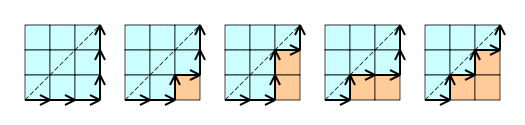
\includegraphics[width=0.4\paperwidth]{./img/catalan.png}
		\caption{\label{fig:hanoi} Látice de tamaño $\left(k,k\right)$.}
	\end{figure}
\end{example}


\begin{example}{La escalera}
	Un niño decide escalar una escalera con $n\geq 1$ de tal manera que cada paso que él despeja uno o dos de los pasos de la escalera %(vea)
	Encuentre la relación de recurrencia que sirva para calcular el número de diferentes maneras posibles de escalar la escalera.
\end{example}
Usamos la variable desconocida $x_{n}$ para denotar el número de maneras en las cuales el niño puede escalar la escalera de $n\geq1$ pasos. Es fácil de observar que $x_{1}=1$ y $x_{2}=2$ (dos pasos cada uno de longitud uno, o un paso de longitud dos escalones). Ahora sea $n\geq3$: si con el primer paso el niño mueve solo el primer escalón; existen claramente $x_{n-1}$ posibles maneras de escalar los que quedan. Si en cambio con el primer lugar, se suben dos peldaños de escalera.
%https://rajsain.files.wordpress.com/2013/11/randomized-algorithms-motwani-and-raghavan.pdf
%
%https://www.csie.ntu.edu.tw/~r97002/temp/Concrete%20Mathematics%202e.pdf
%
%https://link.springer.com/chapter/10.1007/978-3-642-61544-3_9
%
%https://link.springer.com/chapter/10.1007/978-94-011-1814-9_9
%
%https://link.springer.com/chapter/10.1007/978-3-319-15579-1_39
%
%https://link.springer.com/chapter/10.1007/978-94-011-2058-6_14
%
%https://link.springer.com/chapter/10.1007/BFb0120904
%
%https://link.springer.com/chapter/10.1007%2FBFb0120904
%
%https://link.springer.com/article/10.1007/BF00874886
%
%https://link.springer.com/search?date-facet-mode=between&showAll=true&query=recurrence+AND+relation&facet-discipline=%22Mathematics%22

%\motto{hola}
%\runinhead{xd}
%\subruninhead{xd}
%\begin{petit}
%A
%\end{petit}
\subsection{Problemas}

\begin{exercise}
Supongamos que $E_n$ es definido recursivamente en $\mathds{Z}^+$ por \[ E_0=0,E_1=2,\text{ y },E_{n+1}=2n\{E_n+E_{n-1}\} \text{ para }n\geq 1. \] Determine el valor de $E_{10}$.
\end{exercise}

\begin{solution}
	Suponga que $E_{n}$ es definida recursivamente sobre $P$ por \[ E_{0}=0,\quad E_{1}=2,\quad\text{y}\quad E_{n+1}=2n \LEFTRIGHT\{\}{E_{n}+E_{n-1}}\quad\forall n\geq1. \]
	El valor de $E_{10}$ se determina así:
	\begin{align*}
	E_{2}&=E_{1+1}=2(1)\LEFTRIGHT\{\}{E_{1}+E_{0}}=2\LEFTRIGHT\{\}{2+0}=4.\\
	E_{3}&=E_{2+1}=2(2)\LEFTRIGHT\{\}{E_{2}+E_{1}}=4\LEFTRIGHT\{\}{4+2}=24.\\
	E_{4}&=E_{3+1}=2(3)\LEFTRIGHT\{\}{E_{3}+E_{2}}=6\LEFTRIGHT\{\}{24+4}=168.\\
	E_{5}&=E_{4+1}=2(4)\LEFTRIGHT\{\}{E_{4}+E_{3}}=8\LEFTRIGHT\{\}{168+24}=1536.\\
	E_{6}&=E_{5+1}=2(5)\LEFTRIGHT\{\}{E_{5}+E_{4}}=10\LEFTRIGHT\{\}{1536+168}=17040.\\
	E_{7}&=E_{6+1}=2(6)\LEFTRIGHT\{\}{E_{6}+E_{5}}=12\LEFTRIGHT\{\}{17040+1536}=222912.\\
	E_{8}&=E_{7+1}=2(7)\LEFTRIGHT\{\}{E_{7}+E_{6}}=14\LEFTRIGHT\{\}{222912+17040}=3359328.\\
	E_{9}&=E_{8+1}=2(8)\LEFTRIGHT\{\}{E_{8}+E_{7}}=16\LEFTRIGHT\{\}{3359328+222912}=57315840.\\
	E_{10}&=E_{9+1}=2(9)\LEFTRIGHT\{\}{E_{9}+E_{8}}=18\LEFTRIGHT\{\}{57315840+3359328}=1092153024.
	\end{align*}
\end{solution}

\begin{exercise}
Supongamos que la función $f$ es definida recursivamente en $\mathds{Z}^+$ por \[ f(n)\coloneq \ccases{1 & \text{si }n=2^k\text{ para algún }k \in \mathds{N}.\\ f(n/2) & \text{si }n\text{ es par pero no una potencia de 2} \\ f(3n+1) & \text{si }n\text{ es impar.}}. \] Entonces
	\begin{alignat*}{2}
f(3)	=&f(10)	&&\qquad\text{ porque }3\text{ es impar}\\
			=&f(5)	&&\qquad\text{ porque } 10=2\times 5\\
			=&f(16)	&&\qquad\text{ porque }5\text{ es impar}\\
			=&1&&\qquad\text{ porque } 16=2^4.
\end{alignat*}
\begin{enumerate}[(a)]
	\item Mostrar que $f(11)$ también es igual a $1$.
	\item Mostrar que $f(9)$, $f(14)$, y $f(25)$ son todos iguales a $f(11)$ y, por lo tanto, todos iguales a $1$.
	\item Escriba un programa para hallar $f(27)$.
\end{enumerate}
?`Crees que esta función siempre dará el valor de $1$, sin importar con qué $n$ comiences? Busque la ``Conjetura de Collatz'' o el ``Problema del granizo''.
\end{exercise}

\begin{solution}
	
\end{solution}

\begin{exercise}
Podríamos definir una \emph{desajuste} como una $n$--permutación $S$ de $\left\{1,\ldots,n\right\}$ donde cada $S_{j}\neq j$ y luego definir $\bm{D_n}$ como el número de desajustes de $\left\{1,\ldots,n\right\}$. Entonces $D_{n}$ es la única sucesión que satisface la ecuación de recurrencia
\begin{equation}\label{ex:1.3}
D_{n}=\left(n-1\right)\left\{D_{n-1}+D_{n-2}\right\}\text{ para }n=3,4,5,\ldots
\end{equation}
con las condiciones iniciales $D_{1}=0$ y $D_{2}=1$.
\begin{enumerate}[(a)]
	\item Mostrar que $D_{2}=(2)\left(D_{1}\right)+(-1)^2$.
	\item Use la inducción matemática para probar que para todo entero $n\geq2$, \[ D_{n}=(n)(D_{n-1})+{(-1)}^n. \]
\end{enumerate}
\end{exercise}

\begin{solution}

\end{solution}

\begin{exercise}
Use la inducción matemática y la ecuación \eqref{ex:1.3} para probar que \[ \forall n\in\mathds{Z}^{+}\colon\bm{D_n}=n!\sum_{j=0}^n\frac{(-1)^j}{j!}. \]
\end{exercise}

\begin{solution}
	
\end{solution}

\begin{exercise}
Supongamos que (o busque estos dos resultados de cálculo)
\begin{enumerate}[A.]
	\item $\forall x\in\mathds{R}\colon e^x=\sum_{j=0}^\infty\frac{x^j}{j!}$, entonces $e^{-1}=\sum_{j=0}^\infty\frac{(-1)^j}{j!},$
	\item $\forall n\in\mathds{Z}^{+}\colon e^{-1}=\sum_{j=0}^n\frac{(-1)^j}{j!}+E_n$ donde $|E_n|<\left|\frac{(-1)^{n+1}}{(n+1)!}\right|=\frac{1}{(n+1)!}$.
\end{enumerate}

\begin{enumerate}[(a)]
	\item Use el resultado de la pregunta anterior para mostrar \[ \frac{n!}{e}=D_{n}+n!E_{n}\quad\text{donde}\quad|n!E_n|<\frac{n!}{(n+1)!}=\frac{1}{n+1}\leq\frac{1}{2}. \]
	\item Explique por qué $D_{n}-\frac{1}{2}\leq\frac{n!}{e}\leq D_{n}+\frac{1}{2}$.
	\item ?`Es $\left\lceil\frac{n!}{e}\right\rceil=D_{n}$?
\end{enumerate}

\end{exercise}

\begin{solution}
	
\end{solution}

\begin{exercise}
La \emph{función de Ackermann}\index{Ackermann!función} a veces es definida recursivamente en una forma ligeramente diferente
\begin{enumerate}[label={Regla~\arabic*}]
	\item $B\left(0,n\right)=n+1$ para $n=0,1,2,\ldots$,
	\item $B\left(m,0\right)=B\left(m-1,1\right)$ para $m=1,2,3,\ldots$, y
	\item $B\left(m,n\right)=B\left(m-1,B\left(m,n-1\right)\right)$ cuando ambos $m$ y $n$ son positivos.
\end{enumerate}

\begin{enumerate}
	\item Use inducción matemática para probar $\forall n\in\mathds{N}\colon B\left(1,n\right)=n+2$.
	\item Use inducción matemática para probar $\forall n\in\mathds{N}\colon B\left(2,n\right)=3+2n$.
	\item Use inducción matemática para probar $\forall n\in\mathds{N}\colon B\left(3,n\right)=2^{3+n}-3$.
	\item Use inducción matemática para probar $\forall n\in\mathds{N}\colon B\left(4,n\right)=$.
\end{enumerate}
\end{exercise}

\begin{solution}
	
\end{solution}

\begin{exercise}
Supongamos que $A$ es un conjunto de $2n$ objetos. Sea $P_{n}$ el número de diferentes maneras que los objetos en $A$ pueden ser ``emparejados'' (el número de diferentes particiones de $A$ en $2$--subconjuntos). Supongamos que $n\in\mathds{Z}^{+}$. Si $n=2$, entonces $A$ tiene cuatro elementos, $A=\left\{x_1,x_2,x_3,x_4\right\}$. Los tres posibles emparejamientos son:
\begin{enumerate}
	\item $x_{1}$ con $x_{2}$ y $x_{3}$ con $x_{4}$,
	\item $x_{2}$ con $x_{3}$ y $x_{2}$ con $x_{4}$,
	\item $x_{3}$ con $x_{4}$ y $x_{2}$ con $x_{3}$.
\end{enumerate}
Así $P_{2}=3$.

\begin{enumerate}[(a)]% TODO: Crear el programa en Python
	\item Mostrar que si $n=3$ y $A=\left\{x_{1},x_{2},x_{3},x_{4},x_{5},x_{6}\right\}$, existen $15$ posibles emparejamientos enumerándolos a todos:
	\begin{enumerate}
		\item $x_{1}$ con $x_{2}$ y $x_{3}$ con $x_{4}$ y $x_{5}$ con $x_{6}$.
		\item \ldots
	\end{enumerate}
	Así $\bm{P_3}=15$.
	\item Mostrar que $P_{n}$ debe satisfacer la RE $P_{n}=(2n-1)P_{n-1}$ para $\forall n\geq2$.
	\item Use esta ecuación de recurrencia y la inducción matemática para probar \[ P_{n}=\frac{(2n)!}{2^n\times n!}\quad\forall n\geq 1. \]
\end{enumerate}

\end{exercise}

\begin{solution}\leavevmode
	\begin{enumerate}[(a)]
		\item Los $15$ posibles emparejamientos son:
		\begin{enumerate}[1.]
			\item $x_{1}$ con $x_{2}$, $x_{3}$ con $x_{4}$ y $x_{5}$ con $x_{6}$.
			\item $x_{1}$ con $x_{2}$, $x_{3}$ con $x_{5}$ y $x_{4}$ con $x_{6}$.
			\item $x_{1}$ con $x_{2}$, $x_{3}$ con $x_{6}$ y $x_{4}$ con $x_{5}$.
			\item $x_{1}$ con $x_{3}$, $x_{2}$ con $x_{4}$ y $x_{5}$ con $x_{6}$.
			\item $x_{1}$ con $x_{3}$, $x_{2}$ con $x_{5}$ y $x_{4}$ con $x_{6}$.
			\item $x_{1}$ con $x_{2}$, $x_{2}$ con $x_{6}$ y $x_{4}$ con $x_{5}$.
			\item $x_{1}$ con $x_{4}$, $x_{2}$ con $x_{3}$ y $x_{5}$ con $x_{6}$.
			\item $x_{1}$ con $x_{4}$, $x_{2}$ con $x_{5}$ y $x_{3}$ con $x_{6}$.
			\item $x_{1}$ con $x_{4}$, $x_{2}$ con $x_{6}$ y $x_{3}$ con $x_{6}$.
			\item $x_{1}$ con $x_{5}$, $x_{2}$ con $x_{3}$ y $x_{4}$ con $x_{6}$.
			\item $x_{1}$ con $x_{5}$, $x_{2}$ con $x_{4}$ y $x_{3}$ con $x_{6}$.
			\item $x_{1}$ con $x_{5}$, $x_{2}$ con $x_{6}$ y $x_{3}$ con $x_{4}$.
			\item $x_{1}$ con $x_{6}$, $x_{2}$ con $x_{3}$ y $x_{4}$ con $x_{5}$.
			\item $x_{1}$ con $x_{5}$, $x_{2}$ con $x_{4}$ y $x_{3}$ con $x_{5}$.
			\item $x_{1}$ con $x_{6}$, $x_{2}$ con $x_{5}$ y $x_{3}$ con $x_{4}$.
		\end{enumerate}
		Así, $P_{3}=15$ posibles emparejamientos.
		\item Supongamos que $n\geq2$. Un elemento $x_{1}$ puede ser emparejado con cualquier de los $\left(2n-1\right)$ otros elementos en $A$. Esto resulta $2\left(n-2\right)=2\left(n-1\right)$ elementos aún por emparejar, y que pueden emparejarse en $P_{n-1}$ maneras. Así, el número de emparejamientos de $2n$ elementos es $P_{n}=\left(2n-1\right)\times P_{n-1}$.
		\item $P_{n}=(1)(3)\cdots\left(2n-1\right)$, esto es, el producto de los primeros $n$ naturales. Por inducción matemática:
		\begin{enumerate}[label={Paso~\arabic*}]
			\item $P_{1}=1$ que es el primer natural impar.
			\item Asuma que $\exists k\geq1$ donde $P_{k}=(1)(3)\cdots\left(2k-1\right)$.
			\item Si $n=k+1$, entonces para $n\geq2$ y
			\begin{align*}
			P_{k+1}&=\left(2\left[k+1\right]-1\right)P_{j}\quad\text{usando la RE}&\\
			&=\left(2k+1\right)\times(1)(3)\cdots\left(2k-1\right)\quad\text{del paso 2}&\\
			&=(1)(3)(5)\cdots\left(2k-1\right)\times\left(2\left[k+1\right]-1\right).
			\end{align*}
		\end{enumerate}
	\end{enumerate}
\end{solution}


\begin{exercise}
	Mostrar que $y_{n}=\frac{n(n-1)}{2}+c$ para $n>0$ es una solución de la relación de recurrencia \[ y_{n+1}=y_{n}+n. \]
\end{exercise}

\begin{solution}
	$z_{n+1}=\frac{\left[n+1\right]\left(\left[n+1\right]-1\right)}{2}+c=\frac{\left[n+1\right]\left(n\right)}{2}+c=\frac{n\left(n-1\right)+2n}{2}+c=z_{n}+n$.
\end{solution}

\begin{exercise}
Suponga que una sucesión es definida por: \[ f(0)=5\text{ y }f(n+1)=2\times f(n)+1\text{ para } n=0,1,2,\ldots. \]
\begin{enumerate}[(a)]
	\item Encuentre el valor de $f(10)$.
	\item Probar que la sucesión ni es una sucesión aritmética ni es una sucesión geométrica.
\end{enumerate}
\end{exercise}

\begin{solution}
	\begin{enumerate}
		\item
		\begin{align*}
		f(1)&=11, f(2)&=23, f(3)&=47, f(4)&=95, f(5)&=191,\\
		f(6)&=383, f(7)&=767, f(8)&=1535, f(9)&=3071, f(10)&=6143.
		\end{align*}
		\item $f(1)-f(0)=6$, pero $f(2)-f(1)=12$, así que $f$ no es un sucesión aritmética. Por otro lado, $\frac{f(1)}{f(0)}=\frac{11}{5}=\frac{121}{55}$. pero $\frac{f(2)}{f(1)}=\frac{23}{11}=\frac{115}{55}$, por lo tanto, $f$ no es una sucesión geométrica.
	\end{enumerate}
\end{solution}

\begin{exercise}
\begin{enumerate}[(a)]
	\item Encuentre la solución general de la ecuación de recurrencia \[ S_{n}=3S_{n-1}-10\text{ para }n=1,2,\ldots \]\label{ex:1.10a}
	\item Determine la solución particular donde $S_{0}=15$.
	\item Use la fórmula en~\eqref{ex:1.10a} para evaluar $S_6$ y verifique su respuesta usando la ecuación de recurrencia en sí.
\end{enumerate}
\end{exercise}

\begin{solution}
	
\end{solution}

\begin{exercise}
Suponga que $s_{0}=60$ y $s_{n+1}=(1/5)s_n-8$ para $n=0,1,\ldots$.
\begin{enumerate}[(a)]
	\item Encuentre $s_{1}$, $s_{2}$, y $s_{3}$.
	\item Resuelva la relación de recurrencia para dar una fórmula para $s_{n}$.
	\item ?`Es esa sucesión convergente? Si es así, ?`cuál es el límite?
	\item ?`La serie correspondiente converge? Si es así, ?`cuál es el límite?
\end{enumerate}
\end{exercise}

\begin{solution}
	
\end{solution}

\begin{exercise}
Suponga que $s_{0}=75$ y $s_{n+1}=(1/3)s_{n}-6$ para $n=0,1,\ldots$.
\begin{enumerate}[(a)]
	\item Encuentre $s_{1}$, $s_{2}$, y $s_{3}$.
	\item Resuelva la relación de recurrencia para dar una fórmula para $s_{n}$.
	\item ?`Es esa sucesión convergente? Si es así, ?`cuál es el límite?
	\item ?`La serie correspondiente converge? Si es así, ?`cuál es límite?
\end{enumerate}
\end{exercise}

\begin{solution}
	
\end{solution}

\begin{exercise}
\begin{enumerate}[(a)]
	\item Mostrar que $f_{n}=A\times3^{n}+B\times2^{n}$ satisface la ecuación de recurrencia \[ f_{n}=5f_{n-1}-6f_{n-2}\text{ para }n\geq 2. \]
	\item Encuentre la solución particular (valores para $A$ y $B$) para que \[ f_{0}=4\text{ y }f_{1}=17. \]
\end{enumerate}

\end{exercise}

\begin{solution}
	
\end{solution}

\section{Recurrencias Lineales con coeficientes constantes}

Una relación de recurrencia lineal de orden $r$ con coeficientes constantes es una recurrencia del tipo:
\begin{align}\label{1}
c_{0}x_{n}+c_{1}x_{n-1}+\cdots+c_{r}x_{n-r}=h_{n},\forall n\geq r,
\end{align}
donde $c_{0},c_{1},\ldots,c_{r}$ son constantes reales o complejas, con $c_{0}$ y $c_{r}$ ambos diferentes de cero y $(h_{n})_{n\geq r}$ es una sucesión de números reales o complejos llamado sucesión de términos no homogéneos de la recurrencia. La recurrencia es llamada homogénea si la sucesión de términos no homogéneos es una sucesión nula, no homogénea si $h\neq0 $ para algún $n$. La relación de recurrencia:
\begin{align}\label{2}
c_{0}x_{n}+c_{1}x_{n-1}+\cdots+c_{r}x_{n-r}=0,\forall n\geq r,
\end{align}
es llamada la recurrencia homogénea asociada, o la parte homogénea de la recurrencia \eqref{1}. Como nosotros ya hemos notado, la recurrencia:
\begin{equation*}
c_{0}x_{n}+c_{1}x_{n-1}+\cdots+c_{r}x_{n-r}=h_{n},\forall n\geq r,
\end{equation*}
puede ser escrito equivalentemente como
\begin{equation*}
c_{0}x_{n+r}+c_{1}x_{n+(r-1)}+\cdots+c_{r}x_{n}=h_{n+r},\forall n\geq 0.
\end{equation*}
Se puede utilizar cualquiera de las formas presentadas.

\begin{remark}
	Cada $r$-secuencia de valores asignados a las $r$ incógnitas desconocidas de la relación de recurrencia
	\begin{equation*}
	c_{0}x_{n}+c_{1}x_{n-1}+\cdots+c_{r}x_{n-r}=h_{n},\forall n\geq r,
	\end{equation*}
	determina de forma única una solución. Al resolver una relación de recurrencia lineal, el siguiente principio es fundamental importancia.
\end{remark}

\begin{proposition}[Principio de superposición]\index{Principio de superposición}
	Sean ${(u_{n})}_{n}$, ${(V_{n})}_{n}$ respectivamente las soluciones de las relaciones de recurrencia lineal.
	\begin{align*}
	c_{0}x_{n}+c_{1}x_{n-1}+\cdots+c_{r}x_{n-r}&=h_{n},\quad n\geq r
	\intertext{y}
	c_{0}x_{n}+c_{1}x_{n-1}+\cdots+c_{r}x_{n-r}&=k_{n},\quad n\geq r,
	\end{align*}
	con partes homogéneas iguales y secuencias de términos no homogéneos $(h_{n})_{n}$ y $(k_{n})_{n}$. Para cualquier par de constantes $A$ y $B$, la sucesión $(Av_{n}+Bv_{n})_{n}$ es una solución de la relación de recurrencia. \[ c_{0}x_{n}+c_{1}x_{n-1}+\cdots+c_{r}x_{n-r}=Ah_{n}+Bk_{n}. \] La solución general de la relación de recurrencia
	\begin{equation}\label{eq:super}
	c_{0}x_{n}+c_{1}x_{n-1}+\cdots+c_{r}x_{n-r}=h_{n},\quad n\geq r.
	\end{equation}
\end{proposition}

\begin{proof}\leavevmode
	\begin{enumerate}
		\item Uno tiene fácilmente
		\begin{equation*}
		\begin{split}
		&c_{0}(Au_{n}+Bv_{n})+c_{1}(Au_{n-1}+Bv_{n-1})+\cdots+c_{r}(Au_{n-r}+Bv_{n-r})=\\
		&\phantom{c_{0}(Au_n+}=A(c_{0}u_{n}+c_{1}u_{n-1}+\cdots+c_{r}u_{n-r})+B(c_{0}v_{n}+c_{1}v_{n-i}+\cdots+c_{r}v_{n-r})\\
		&\phantom{c_{0}(Au_n+}=Ah_{n}+Bk_{n}.
		\end{split}
		\end{equation*}
		\item Sea $(u_{n})_{n}$ una solución particular de \eqref{eq:super}. Por el punto previo nosotros conocemos que $(v_{n})_{n}=(u_{n})_{n}+(v_{n}-u_{n})_{n}$ es una solución de \eqref{eq:super} si y solo si $v_{n}-u_{n}$ es una solución de la recurrencia homogénea asociada. Por lo tanto cada solución de \eqref{eq:super} es obtenida añadiendo una solución de la  recurrencia homogénea asociada para $(u_{n})_{n}$.
	\end{enumerate}
\end{proof}

\section{Relación de recurrencia lineal con homogénea con coeficientes constantes}

La sucesión nula es una solución de cualquier relación de recurrencia lineal. La estructura de la solución general de una relación de recurrencia lineal homogénea corresponde a la estructura de la solución general de un sistema de ecuaciones lineales homogéneas.
\begin{proposition}[Teorema principal]
	Considere la relación de recurrencia lineal homogénea de orden $r$:
	\begin{equation}\label{eq:homo}
	c_{0}x_{n}+c_{1}x_{n-1}+\cdots+c_{r}x_{n-r}=0,\quad n\geq r\quad\left(c_{0}c_{r}\neq0\right)
	\end{equation}
	\begin{enumerate}
		\item Cualquier combinación lineal de soluciones de \eqref{eq:homo} es de nuevo una solución de \eqref{eq:homo}.
		\item Existe $r$ soluciones de \eqref{eq:homo} tal que cualquier otra solución de \eqref{eq:homo} puede ser expresado únicamente como su combinación lineal.
	\end{enumerate}
\end{proposition}

\begin{proof}\leavevmode
	\begin{enumerate}
		\item Esto sigue inmediatamente por el ``Principio de Superposición''.
		\item Para todo $i\in\left\{0,\ldots,r-1 \right\}$ sea $\left(u^{i}_{n}\right)_{n}$ la solución de \eqref{eq:homo} con $r$--sucesión de valores iniciales iguales a $0$ para índices $j\neq i$, iguales a $1$ en índices $i$, es decir: \[ u^{i}_{j}=0\text{ si }j\neq i,\quad u^{i}_{i}=1\quad j\in\left\{0,\ldots,r-1 \right\}. \]
		Consideramos ahora alguna solución $(a_{n})_{n}$ de \eqref{eq:homo}; la combinación lineal \[ a_{0}{\left(u^{0}_{n}\right)}_{n}+a_{1}{\left(u^{1}_{n}\right)}_{n}+\cdots+a_{r-1}(u^{r-1}_{n})_{n}, \]	es una solución de \eqref{eq:homo} con secuencia de datos iniciales $\left(a_{0},\ldots,a_{r-1}\right)$. Ya que la sucesión de valores iniciales determinan la solución de una relación de recurrencia, uno tiene \[ {\left(a_{n}\right)}_{n}=a_{0}\left(u^{0}_{n}\right)_{n}+a_{1}\left(u^{1}_{n}\right)_{n}+\cdots+a_{r-1}\left(u^{r-1}_{n}\right)_{n}. \]
	\end{enumerate}
\end{proof}

\begin{definition}[Polinomio característico]\index{Relación de recurrencia!polinomio característico}
	Definimos el \emph{polinomio característico} de una relación de recurrencia con coeficientes constantes de orden $r$ de la siguiente manera: \[ c_{0}x_{n}+c_{1}x_{n-1}+\cdots+c_{r}x_{n-r}=h_{n},\quad n\geq r\left(c_{0}c_{r}\neq0\right), \] para el polinomio de grado $r$: \[ P(X)\coloneqq c_{0}X^{r}+c_{1}X^{r-1}+\cdots+c_{r}. \] Cada polinomio de grado $r$ tiene exactamente $r$ raíces complejas contando con su multiplicidad. Vemos ahora que la sucesión de las potencias naturales de una determinada raíz del polinomio característico de una relación de recurrencia lineal es una solución de la correspondiente relación homogénea.
\end{definition}

\begin{proposition}[Raíz del polinomio característico]\index{Relación de recurrencia!polinomio característico!raíz}
	Sea $\lambda\in\mathds{C}$. La sucesión $\left(\lambda^{n}\right)_{n}$ de las potencias de $\lambda$ es una solución de la relación de recurrencia lineal homogénea
	\begin{align}\label{5}
	c_{0}x_{n}+c_{1}x_{n-1}+\cdots+c_{r}x_{n-r}=0,\quad n\leq r \quad (c_{0}c_{r}\neq 0),
	\end{align}
	sii $\lambda$ es una raíz de este polinomio característico.
\end{proposition}

\begin{proof}
	Dado que $c_{r}\neq0$, las raíces del polinomio característico deben ser necesariamente no nulas. Sustituyendo los valores de la sucesión ${\left(\lambda^{n}\right)}_{n}$ en la recurrencia, uno tiene \[ c_{0}x_{n}+c_{1}x_{n-1}+\cdots+c_{r}x_{n-r}=0, \] y dividiendo por $\lambda^{n-r}\neq0$ \[ c_{0}\lambda^{r}+c_{1}\lambda^{r-1}+\cdots+c_{r}=0. \]	Por lo tanto, la sucesión ${\left(\lambda^{n}\right)}_{n}$ es una solución de \eqref{5} sii $\lambda$ es una raíz del polinomio $c_{0}X^{r}+c_{1}X^{r-1}+\cdots+c_{r}$.
\end{proof}

En general, no es fácil encontrar las raíces de un polinomio de grado mayor que dos, aunque uno puede siempre usar un adecuado CAS. El siguiente criterio simple, sin embargo, muestra cómo encontrar las raíces racionales de un polinomio con coeficientes enteros.

\begin{proposition}[Las raíces racionales de un polinomio con coeficientes enteros]
	Sea $P(X)=c_{0}X^{r}+c_{1}X^{r-1}+\cdots+c_{r}$ un polinomio con coeficientes enteros $c_{0}\ldots c_{r}\in\mathds{Z}$, con $c_{0}\neq 0$. Si la fracción $\tfrac{a}{b}$ con $a,b\in\mathds{Z}$ con $\operatorname{mcd}=1$ es una raíz de $P(X)$, luego $a\divides c_{r}$ y $b\divides c_{0}$. En particular, si $c_{0}=\pm1$ las raíces racionales del polinomio $P(X)$ son enteros que dividen a $c_{r}$.
\end{proposition}

\begin{proof}
	Dado $c_{0}\left(\frac{a}{b}\right)^{r}+c_{1}{\left(\frac{a}{b}\right)}^{r-1}+\cdots+c_{r-1}\left(\frac{a}{b}\right)+c_{r}=0$, multiplicado por $b^{r}$ obtenemos: \[ 	c_{0}a^{r}+c_{1}a^{r-1}b+\cdots+c_{r-1}ab^{r-1}+c_{r}b^{r}=0. \] Como $a\divides c_{0}a^{r}+c_{1}a^{r-1}b+\cdots+c_{r-1}ab^{r-1}$, luego tiene que dividir también $c_{r}b^{r}$, y por lo tanto, al no tener $a$ y $b$ factores comunes, $a\divides c_{r}$. Análogamente $b\divides c_{0}a^{r}$ y por lo tanto divide a $c_{0}$.
\end{proof}

\begin{example}{Polinomio característico}
	La recurrencia homogénea de segundo orden: \[ x_{n}=2x_{n-1}-2x_{n-2},\quad n\geq2, \] tiene polinomio característico $X^{2}-2X+2$ cuyas raíces son $\lambda_{1}=1-i$ y $\lambda_{2}=1+i$. Las sucesiones ${\left((1-i)^{n}\right)}_{n}$ y ${\left((1+i)^{n}\right)}_{n} $ son las soluciones bases de la recurrencia. La solución general compleja de la recurrencia es: \[ x_{n}=A_{1}{\left(1-i\right)}^{n}+A_{2}{\left(1+i\right)}^{n},\quad n\geq 0, \] con la variante de $A_{1}$ y $A_{2}$ entre los números complejos. Veamos la solución real general. Uno tiene: \[ \lambda_{1}=1-i=\sqrt{2}\left(\frac{\sqrt{2}}{2}-\frac{\sqrt{2}}{2}i\right)=\sqrt{2}\left(\cos\left(\frac{\pi}{4}\right)-i\sen\left(\frac{\pi}{4}\right)\right) \] y \[ \lambda_{2}=1+i=\overline{\lambda_{1}}=\sqrt{2}\left(\cos\left(\frac{\pi}{4}\right)-i\sen\left(\frac{\pi}{4}\right)\right). \] Luego, las sucesiones ${\left(2^{n/2}\cos\left( \frac{n\pi}{4}\right)\right)}_{n}$ y ${\left(2^{n/2}\sen\left(\frac{n\pi}{4}\right)\right)}_{n}$ son las soluciones base reales de la recurrencia. Por lo tanto, la solución general real de la recurrencia es: \[ x_{n}=A_{1}2^{n/2}\cos\left(\frac{n\pi}{4}\right)+A_{2}2^{n/2}\sen\left(\frac{n\pi}{4}\right),\quad n\geq 0, \] con la variación de $A_{1}$ y $A_{2}$ entre los números reales.
\end{example}

\begin{claim}
Afirmo que el Lema de Zorn es cierto.
\end{claim}

\begin{proof}
$\smartqed$

$\qed$
\end{proof}

\begin{case}
	
\end{case}

\begin{conjecture}
	
\end{conjecture}

\begin{corollary}
	
\end{corollary}

\begin{definition}
	
\end{definition}

\begin{example}{Quispe}
	
\end{example}

\begin{lemma}
	
\end{lemma}

\begin{note}
	
\end{note}

\begin{problem}
	
\end{problem}

\begin{property}
	
\end{property}

\begin{proposition}
	
\end{proposition}

\begin{question}{Bryan}
	
\end{question}

\begin{remark}

\end{remark}

\begin{theorem}

\end{theorem}

\begin{trailer}{Enfatizar párrafos}
\end{trailer}

\begin{question}{?`Qué hora es?}
\end{question}

\begin{important}{Importante}
	A
\end{important}

\begin{warning}{Atención}
	
\end{warning}

\begin{tips}{Consejos}
	
\end{tips}

\begin{overview}{Enfatizar párrafos completos}
	
\end{overview}

\begin{backgroundinformation}{Información de fondo}
	
\end{backgroundinformation}

\begin{legaltext}{Texto legal}
	
\end{legaltext}